% ============================================================
% Question Bank: ch02-06 Simple Interest
% Topic Title: Simple Interest: Earning and Paying Interest
% CCSS: 7.RP.A.3
% Questions: 27 (15 MC + 6 SA + 6 Graphical)
% ============================================================

% --- Multiple Choice Questions (15) ---

\begin{practiceQuestion}{2-6-q01}{mc}
\begin{questionText}
Find the simple interest earned on $\$900$ at $3\%$ per year for $4$ years.
\end{questionText}
\choiceA{$\$27$}
\choiceB{$\$36$}
\choiceC{$\$108$}
\choiceD{$\$120$}
\correctAnswer{C}
\explanation{Use the simple interest formula $I = Prt$: $I = 900 \times 0.03 \times 4 = \$108$.}
\end{practiceQuestion}

\begin{practiceQuestion}{2-6-q02}{mc}
\begin{questionText}
You deposit $\$1{,}500$ at $5\%$ simple interest for $3$ years. What is the total amount in your account?
\end{questionText}
\choiceA{$\$225$}
\choiceB{$\$1{,}575$}
\choiceC{$\$1{,}650$}
\choiceD{$\$1{,}725$}
\correctAnswer{D}
\explanation{$I = 1{,}500 \times 0.05 \times 3 = \$225$. Total: $1{,}500 + 225 = \$1{,}725$.}
\end{practiceQuestion}

\begin{practiceQuestion}{2-6-q03}{mc}
\begin{questionText}
A student writes $I = 700 \times 4 \times 2 = \$5{,}600$. What mistake did the student make?
\end{questionText}
\choiceA{Switched $P$ and $t$}
\choiceB{Used the wrong formula}
\choiceC{Forgot to convert $4\%$ to a decimal}
\choiceD{Divided instead of multiplied}
\correctAnswer{C}
\explanation{The rate $4\%$ must be written as $0.04$. Correct: $I = 700 \times 0.04 \times 2 = \$56$.}
\end{practiceQuestion}

\begin{practiceQuestion}{2-6-q04}{mc}
\begin{questionText}
You borrow $\$2{,}400$ at $7\%$ simple interest for $3$ years. How much interest do you owe?
\end{questionText}
\choiceA{$\$168$}
\choiceB{$\$336$}
\choiceC{$\$504$}
\choiceD{$\$720$}
\correctAnswer{C}
\explanation{$I = 2{,}400 \times 0.07 \times 3 = \$504$.}
\end{practiceQuestion}

\begin{practiceQuestion}{2-6-q05}{mc}
\begin{questionText}
A savings account earns $2.5\%$ simple interest per year. You deposit $\$800$. After how many years will you earn $\$100$ in interest?
\end{questionText}
\choiceA{$4$ years}
\choiceB{$5$ years}
\choiceC{$8$ years}
\choiceD{$10$ years}
\correctAnswer{B}
\explanation{$100 = 800 \times 0.025 \times t$. Simplify: $100 = 20t$, so $t = 5$ years.}
\end{practiceQuestion}

\begin{practiceQuestion}{2-6-q06}{mc}
\begin{questionText}
Which investment earns more interest: $\$1{,}200$ at $3\%$ for $5$ years, or $\$1{,}200$ at $5\%$ for $3$ years?
\end{questionText}
\choiceA{$3\%$ for $5$ years --- $\$180$}
\choiceB{$5\%$ for $3$ years --- $\$180$}
\choiceC{They earn the same interest}
\choiceD{Cannot be determined}
\correctAnswer{C}
\explanation{First: $1{,}200 \times 0.03 \times 5 = \$180$. Second: $1{,}200 \times 0.05 \times 3 = \$180$. They are equal.}
\end{practiceQuestion}

\begin{practiceQuestion}{2-6-q07}{mc}
\begin{questionText}
A car loan of $\$5{,}000$ charges $\$900$ in interest over $3$ years. What is the annual interest rate?
\end{questionText}
\choiceA{$3\%$}
\choiceB{$5\%$}
\choiceC{$6\%$}
\choiceD{$9\%$}
\correctAnswer{C}
\explanation{$900 = 5{,}000 \times r \times 3$. So $15{,}000r = 900$ and $r = 0.06 = 6\%$.}
\end{practiceQuestion}

\begin{practiceQuestion}{2-6-q08}{mc}
\begin{questionText}
You deposit $\$650$ at $4\%$ simple interest. What is the total after $5$ years?
\end{questionText}
\choiceA{$\$130$}
\choiceB{$\$680$}
\choiceC{$\$750$}
\choiceD{$\$780$}
\correctAnswer{D}
\explanation{$I = 650 \times 0.04 \times 5 = \$130$. Total: $650 + 130 = \$780$.}
\end{practiceQuestion}

\begin{practiceQuestion}{2-6-q09}{mc}
\begin{questionText}
Mia deposits $\$400$ at $6\%$. Carlos deposits $\$600$ at $4\%$. Both save for $2$ years. Who earns more interest and by how much?
\end{questionText}
\choiceA{Mia earns $\$48$; Carlos earns $\$48$ --- tied}
\choiceB{Mia earns $\$48$; Carlos earns $\$24$ --- Mia by $\$24$}
\choiceC{Mia earns $\$24$; Carlos earns $\$48$ --- Carlos by $\$24$}
\choiceD{They cannot be compared}
\correctAnswer{A}
\explanation{Mia: $400 \times 0.06 \times 2 = \$48$. Carlos: $600 \times 0.04 \times 2 = \$48$. They are tied.}
\end{practiceQuestion}

\begin{practiceQuestion}{2-6-q10}{mc}
\begin{questionText}
A student borrows $\$1{,}000$ at $8\%$ and pays a total of $\$1{,}320$. How many years was the loan?
\end{questionText}
\choiceA{$2$ years}
\choiceB{$3$ years}
\choiceC{$4$ years}
\choiceD{$5$ years}
\correctAnswer{C}
\explanation{Interest paid: $1{,}320 - 1{,}000 = \$320$. Solve: $320 = 1{,}000 \times 0.08 \times t$, so $80t = 320$ and $t = 4$ years.}
\end{practiceQuestion}

\begin{practiceQuestion}{2-6-q11}{mc}
\begin{questionText}
In the formula $I = Prt$, if you double the time, what happens to the interest?
\end{questionText}
\choiceA{It stays the same}
\choiceB{It doubles}
\choiceC{It triples}
\choiceD{It is halved}
\correctAnswer{B}
\explanation{Since $I = Prt$, doubling $t$ while keeping $P$ and $r$ the same doubles the interest. The formula is directly proportional to time.}
\end{practiceQuestion}

\begin{practiceQuestion}{2-6-q12}{mc}
\begin{questionText}
You deposit $\$3{,}000$ at $2\%$ simple interest for $6$ months. How much interest do you earn?
\end{questionText}
\choiceA{$\$30$}
\choiceB{$\$36$}
\choiceC{$\$60$}
\choiceD{$\$360$}
\correctAnswer{A}
\explanation{$6$ months $= 0.5$ years. $I = 3{,}000 \times 0.02 \times 0.5 = \$30$.}
\end{practiceQuestion}

\begin{practiceQuestion}{2-6-q13}{mc}
\begin{questionText}
A loan of $\$4{,}000$ at $3.5\%$ simple interest runs for $2$ years. What is the total amount owed?
\end{questionText}
\choiceA{$\$140$}
\choiceB{$\$4{,}140$}
\choiceC{$\$4{,}280$}
\choiceD{$\$4{,}700$}
\correctAnswer{C}
\explanation{$I = 4{,}000 \times 0.035 \times 2 = \$280$. Total: $4{,}000 + 280 = \$4{,}280$.}
\end{practiceQuestion}

\begin{practiceQuestion}{2-6-q14}{mc}
\begin{questionText}
A bank pays $\$112.50$ in interest on a $\$1{,}500$ deposit over $3$ years. What is the annual rate?
\end{questionText}
\choiceA{$2\%$}
\choiceB{$2.5\%$}
\choiceC{$3\%$}
\choiceD{$3.5\%$}
\correctAnswer{B}
\explanation{$112.50 = 1{,}500 \times r \times 3$. So $4{,}500r = 112.50$ and $r = 0.025 = 2.5\%$.}
\end{practiceQuestion}

\begin{practiceQuestion}{2-6-q15}{mc}
\begin{questionText}
Aliyah wants to earn at least $\$200$ in interest. She deposits $\$2{,}500$ at $4\%$. What is the minimum number of whole years she must save?
\end{questionText}
\choiceA{$1$ year}
\choiceB{$2$ years}
\choiceC{$3$ years}
\choiceD{$4$ years}
\correctAnswer{B}
\explanation{$200 = 2{,}500 \times 0.04 \times t$. So $100t = 200$ and $t = 2$ years.}
\end{practiceQuestion}

% --- Short Answer Questions (6) ---

\begin{practiceQuestion}{2-6-q16}{sa}
\begin{questionText}
Find the simple interest on $\$1{,}800$ at $3.5\%$ for $4$ years.
\end{questionText}
\correctAnswer{$\$252$}
\explanation{$I = 1{,}800 \times 0.035 \times 4 = \$252$.}
\end{practiceQuestion}

\begin{practiceQuestion}{2-6-q17}{sa}
\begin{questionText}
You borrow $\$950$ at $6\%$ for $2$ years. What is the total amount you must pay back?
\end{questionText}
\correctAnswer{$\$1{,}064$}
\explanation{$I = 950 \times 0.06 \times 2 = \$114$. Total: $950 + 114 = \$1{,}064$.}
\end{practiceQuestion}

\begin{practiceQuestion}{2-6-q18}{sa}
\begin{questionText}
A deposit of $\$2{,}000$ earns $\$300$ in interest at $5\%$. How many years was the money deposited?
\end{questionText}
\correctAnswer{$3$ years}
\explanation{$300 = 2{,}000 \times 0.05 \times t$. So $100t = 300$ and $t = 3$ years.}
\end{practiceQuestion}

\begin{practiceQuestion}{2-6-q19}{sa}
\begin{questionText}
You deposit $\$4{,}000$ at $1.5\%$ for $2$ years. How much interest do you earn?
\end{questionText}
\correctAnswer{$\$120$}
\explanation{$I = 4{,}000 \times 0.015 \times 2 = \$120$.}
\end{practiceQuestion}

\begin{practiceQuestion}{2-6-q20}{sa}
\begin{questionText}
A loan of $\$6{,}000$ at $4.5\%$ charges $\$810$ in interest. How many years was the loan?
\end{questionText}
\correctAnswer{$3$ years}
\explanation{$810 = 6{,}000 \times 0.045 \times t$. So $270t = 810$ and $t = 3$ years.}
\end{practiceQuestion}

\begin{practiceQuestion}{2-6-q21}{sa}
\begin{questionText}
Which earns more interest: $\$500$ at $8\%$ for $1$ year, or $\$500$ at $2\%$ for $4$ years?
\end{questionText}
\correctAnswer{They earn the same ($\$40$)}
\explanation{First: $500 \times 0.08 \times 1 = \$40$. Second: $500 \times 0.02 \times 4 = \$40$. They are equal.}
\end{practiceQuestion}

% --- Graphical Questions (3 GMC + 3 GSA) ---

\begin{practiceQuestion}{2-6-q22}{gmc}
\begin{questionText}
The table shows three savings plans. Which plan earns the most interest?

\begin{center}
\begin{tabular}{|l|c|c|c|}
\hline
\textbf{Plan} & \textbf{Principal} & \textbf{Rate} & \textbf{Years} \\
\hline
A & $\$1{,}000$ & $4\%$ & $3$ \\
\hline
B & $\$800$ & $5\%$ & $3$ \\
\hline
C & $\$1{,}500$ & $2\%$ & $4$ \\
\hline
\end{tabular}
\end{center}
\end{questionText}
\choiceA{Plan A ($\$120$)}
\choiceB{Plan B ($\$120$)}
\choiceC{Plan C ($\$120$)}
\choiceD{All three earn the same}
\correctAnswer{D}
\explanation{A: $1{,}000 \times 0.04 \times 3 = \$120$. B: $800 \times 0.05 \times 3 = \$120$. C: $1{,}500 \times 0.02 \times 4 = \$120$. All earn $\$120$.}
\end{practiceQuestion}

\begin{practiceQuestion}{2-6-q23}{gmc}
\begin{questionText}
The line graph shows the total amount in a simple interest savings account over time. What is the annual interest rate?

\begin{center}
\begin{tikzpicture}[scale=0.7]
  \draw[thick,->] (0,0) -- (6,0) node[right]{\small Years};
  \draw[thick,->] (0,0) -- (0,5.5) node[above]{\small Amount (\$)};
  \foreach \x in {0,...,5} {
    \draw (\x,-0.1) -- (\x,0.1) node[below=3pt,font=\small] {\x};
  }
  \foreach \y/\lab in {1/200,2/400,3/600,4/800,5/1000} {
    \draw (-0.1,\y) -- (0.1,\y) node[left,font=\small,xshift=-2pt] {\lab};
  }
  \draw[thick,funBlue,mark=*,mark size=2pt] plot coordinates {(0,2.5) (1,2.75) (2,3) (3,3.25) (4,3.5) (5,3.75)};
  \node[right,font=\small,funBlue] at (5,3.75) {$\$750$};
  \node[left,font=\small,funBlue] at (0,2.5) {$\$500$};
\end{tikzpicture}
\end{center}
\end{questionText}
\choiceA{$5\%$}
\choiceB{$8\%$}
\choiceC{$10\%$}
\choiceD{$25\%$}
\correctAnswer{C}
\explanation{Principal: $\$500$. After $5$ years: $\$750$. Interest: $750 - 500 = \$250$. Rate: $250 \div (500 \times 5) = 250 \div 2{,}500 = 0.10 = 10\%$.}
\end{practiceQuestion}

\begin{practiceQuestion}{2-6-q24}{gmc}
\begin{questionText}
The bar graph compares the interest earned by two accounts over the same period. Account A has $\$2{,}000$ at $3\%$. Account B has $\$1{,}000$ at what rate, if both earn the same interest after $4$ years?

\begin{center}
\begin{tikzpicture}[scale=0.5]
  \draw[thick,->] (0,0) -- (0,5.5) node[above]{\small Interest (\$)};
  \draw[thick,->] (0,0) -- (6,0);
  \fill[funBlue!60] (0.75,0) rectangle (2.25,4);
  \fill[funGreen!60] (3.25,0) rectangle (4.75,4);
  \node[below,font=\small] at (1.5,0) {Acct A};
  \node[below,font=\small] at (4,0) {Acct B};
  \foreach \y/\lab in {1/60,2/120,3/180,4/240} {
    \draw (-0.1,\y) -- (0.1,\y) node[left,font=\small,xshift=-2pt] {\lab};
  }
  \node[above,font=\small] at (1.5,4) {$\$240$};
  \node[above,font=\small] at (4,4) {$\$240$};
\end{tikzpicture}
\end{center}
\end{questionText}
\choiceA{$3\%$}
\choiceB{$4\%$}
\choiceC{$6\%$}
\choiceD{$8\%$}
\correctAnswer{C}
\explanation{Account A: $2{,}000 \times 0.03 \times 4 = \$240$. Account B: $240 = 1{,}000 \times r \times 4$, so $4{,}000r = 240$ and $r = 0.06 = 6\%$.}
\end{practiceQuestion}

\begin{practiceQuestion}{2-6-q25}{gsa}
\begin{questionText}
The timeline below shows a loan. Find the total amount owed at the end.

\begin{center}
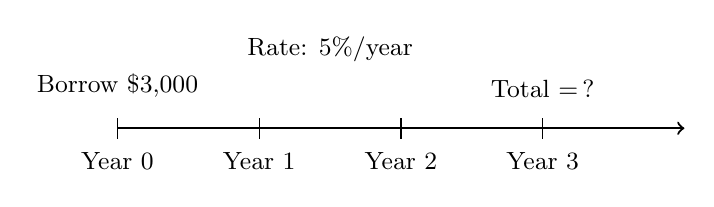
\begin{tikzpicture}[scale=0.9]
  \draw[thick,->] (0,0) -- (8,0);
  \foreach \x/\lab in {0/Year 0, 2/Year 1, 4/Year 2, 6/Year 3} {
    \draw (\x,-0.15) -- (\x,0.15);
    \node[below,font=\small] at (\x,-0.2) {\lab};
  }
  \node[above,font=\small] at (0,0.3) {Borrow $\$3{,}000$};
  \node[above,font=\small] at (3,0.8) {Rate: $5\%$/year};
  \node[above,font=\small] at (6,0.3) {Total $= \,?$};
\end{tikzpicture}
\end{center}
\end{questionText}
\correctAnswer{$\$3{,}450$}
\explanation{$I = 3{,}000 \times 0.05 \times 3 = \$450$. Total: $3{,}000 + 450 = \$3{,}450$.}
\end{practiceQuestion}

\begin{practiceQuestion}{2-6-q26}{gsa}
\begin{questionText}
The table below shows two deposit options. How much more total money does Option B give after the stated time?

\begin{center}
\begin{tabular}{|l|c|c|c|}
\hline
 & \textbf{Principal} & \textbf{Rate} & \textbf{Time} \\
\hline
Option A & $\$2{,}000$ & $3\%$ & $4$ years \\
\hline
Option B & $\$2{,}000$ & $5\%$ & $4$ years \\
\hline
\end{tabular}
\end{center}
\end{questionText}
\correctAnswer{$\$160$}
\explanation{Option A interest: $2{,}000 \times 0.03 \times 4 = \$240$. Option B interest: $2{,}000 \times 0.05 \times 4 = \$400$. Difference: $400 - 240 = \$160$.}
\end{practiceQuestion}

\begin{practiceQuestion}{2-6-q27}{gsa}
\begin{questionText}
The bar graph below shows the interest earned each year on a $\$1{,}000$ deposit. Since simple interest is the same each year, how many years does it take to earn a total of $\$350$?

\begin{center}
\begin{tikzpicture}[scale=0.55]
  \draw[thick,->] (0,0) -- (0,4.5) node[above]{\small Interest (\$)};
  \draw[thick,->] (0,0) -- (5,0);
  \fill[funOrange!60] (1,0) rectangle (2.5,3.5);
  \node[below,font=\small] at (1.75,0) {Year 1};
  \node[above,font=\small] at (1.75,3.5) {$\$70$};
  \foreach \y/\lab in {1/20,2/40,3/60,3.5/70} {
    \draw (-0.1,\y) -- (0.1,\y) node[left,font=\small,xshift=-2pt] {\lab};
  }
  \node[font=\small] at (3.5,2) {Same each year};
\end{tikzpicture}
\end{center}
\end{questionText}
\correctAnswer{$5$ years}
\explanation{Each year earns $\$70$. To reach $\$350$: $350 \div 70 = 5$ years.}
\end{practiceQuestion}
